\subsection{UC2 - Selezione dimensioni da utilizzare}
\begin{figure}[h]
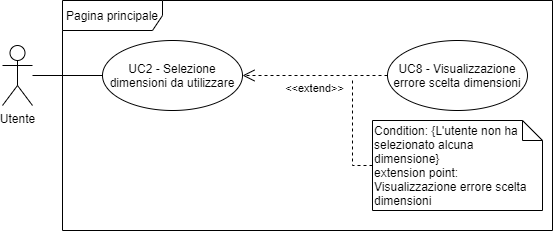
\includegraphics[width=\linewidth]{Section/Images/UC2.png}
\centering
\caption{UC2 - Selezione dimensioni da analizzare}
\end{figure}
\begin{itemize}
	\item \textbf{Attore primario}: Utente.
	\item \textbf{Precondizioni}: L'utente ha caricato i dati nel sistema [UC1].
	\item \textbf{Postcondizioni}: Le dimensioni scelte vengono memorizzate nel sistema e i dati sono pronti per essere visualizzati [UC5].
	\item \textbf{Scenario principale}:
		\begin{enumerate}
			\item All'utente viene presentata una schermata con tutte le dimensioni presenti nel dataset caricato;
			\item Per ogni dimensione è presente una cella da selezionare nel caso la si voglia utilizzare;
			\item L'utente seleziona le dimensioni che desidera analizzare;
		\end{enumerate}
	\item \textbf{Estensioni:}
		\begin{enumerate}[(a)]
			\item Nel caso in cui l'utente non abbia selezionato nessuna dimensione:
			\begin{enumerate}[1.]
				\item Le dimensioni non vengono memorizzate nel sistema;
				\item Viene visualizzato un messaggio d'errore esplicativo [UC10].
			\end{enumerate}
		\end{enumerate}
\end{itemize}